\documentclass[
	11pt, 
	DIV10,
	a4paper, 
	oneside, 
	headings=normal, 
	captions=tableheading,
	final, 
	numbers=noenddot
]{scrartcl}

\usepackage{lipsum}
\usepackage{graphicx}
\usepackage{amsmath}
\usepackage{mathtools}
\usepackage{amssymb}
\usepackage{bm}
\usepackage[utf8]{inputenc}





\title{Example-based Plastic Deformation of Rigid Bodies}
\subtitle{\vspace{0.5cm}Seminar: Current Topics in Physically-Based Animation}
\author{Younes Müller}


\begin{document}
\maketitle
\tableofcontents
\newpage


\section{Introduction}
In modern days, computer graphics gains a lot of importance. David Kriesel once stated in one of his talks that the eye is the only broad band connection to the brain \cite{dkriesel}. So the eye is the way to go to provide much detailed information to humans.
Despite the large computational effort the results need to be computed nearly in real time for games and VR applications.\\
The field of physically based animation tightly belongs to computer graphics. A method to efficiently simulate the physical movement of objects is rigid body simulation. It assumes that the objects' shape is unchangeable This results in very fast computations. As the name suggests deformation of objects is not simulated during rigid body simulation
In this seminar work I will describe and explain a method to solve this problem, described by Ben Jones, Niles Thuerey, Tamar Shinar and Adam W. Bargteil in their article "Example-based Plastic Deformation of Rigid Bodies."\cite{paper}
They developed a method, that extends a rigid body simulator. It is based on deformation example poses.
A set of example deformations are provided by an artist or a soft body simulation. Additionally to the speed of this method it gives the user the ability to control exactly, how the deformed bodies look. 
\section{Method}
\begin{figure}[tb]
	\centering
	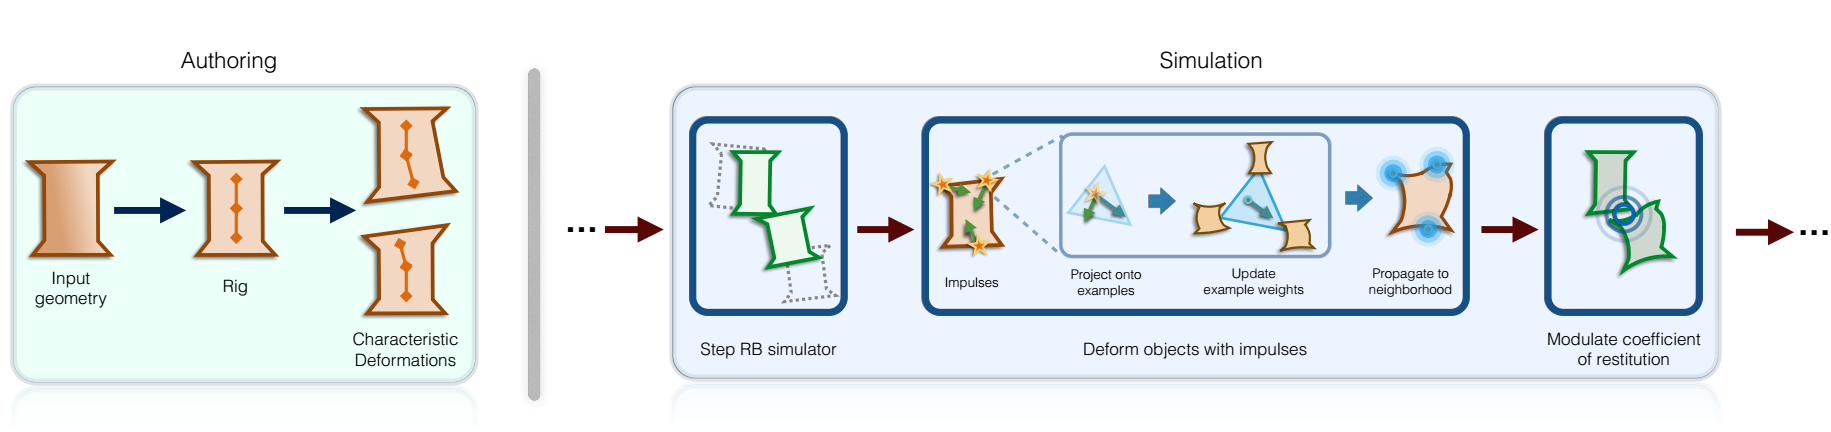
\includegraphics[width=0.8\linewidth]{images/process} 	
	\caption{\label{fig:process} Overview of the authoring and simulation process.\cite{paper}
	}
\end{figure}

\subsection{Overview}
Figure \ref{fig:process} Gives an overview over the method.
During the authoring, the artist provides a set of example poses with the help of bones.
The simulation step is done each time the rigid body simulator detects a collision. It hands the collision impulses to our routine. We then calculate a combination of the given examples that matches the deformation best. Then the combination is propagated towards the nearby vertices. To increase physical correctness, the non elastic part of the collision is increased.

\subsection{Example}
In Figure \ref{fig:ex1} we have a mesh and one example pose. The third image visualizes which vertex positions can be reached through blending of the example and the mesh.\\
\begin{figure}[tb]
	\centering
	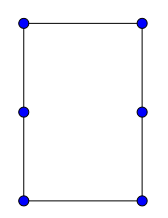
\includegraphics[height=.3\linewidth]{images/ex1} 	
	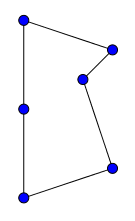
\includegraphics[height=.31\linewidth]{images/ex2} 	
	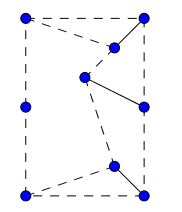
\includegraphics[height=.31\linewidth]{images/ex5} 	
	\caption{\label{fig:ex1} 1. the mesh 2. the example pose 3. the example space}
\end{figure}
Figure \ref{fig:ex2}: The barrel collides with another object. Now the impulse $\bm j_i$ is acting upon vertex $\bm{x_i}$. An ideal change in position $\bm{\Delta x}$ is calculated.\\
\begin{figure}[tb]
	\centering
	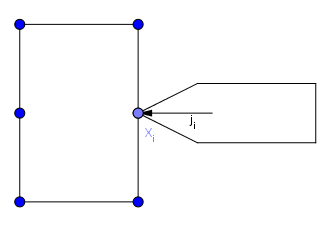
\includegraphics[height=.3\linewidth]{images/ex3} 	
	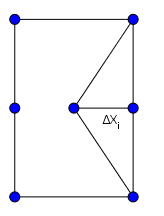
\includegraphics[height=.31\linewidth]{images/ex4} 	
	\caption{\label{fig:ex2} 1. the impulse j 2. the initial change}
\end{figure}
Figure \ref{fig:ex3}: The ideal change $\bm{\Delta x}$ moves the vertex $\bm{x}$ out of the example space. So an example weighting is calculated, which matches the position best. Afterwards the change is propagated to the nearby vertices. The higher the distance to the hit vertex $\bm{x}$, the less impact the change has on the vertex.
\begin{figure}[tb]
	\centering
	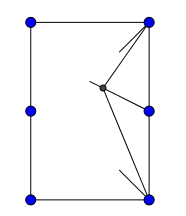
\includegraphics[height=.3\linewidth]{images/ex6} 	
	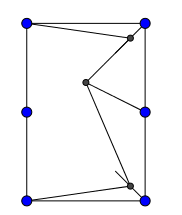
\includegraphics[height=.31\linewidth]{images/ex7} 	
	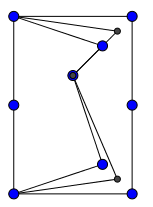
\includegraphics[height=.31\linewidth]{images/ex8} 	
	\caption{\label{fig:ex3} 1. approximated $\bm{\Delta x}$ in example space 2. the propagated change in example space 3. mesh, example and blend}
\end{figure}

\subsection{Rigid Bodies}
\cite{lecRigidBodies} To simulate the translational motion of a rigid body it is sufficient to simulate the motion of the center of mass. As the vertices stay motionless relative to the center the position of every vertex can be calculated easily from the position of the center. 
If the motion is arbitrary it can still be represented by just a translational and a rotational movement. 
The simulation is done by a rigid body simulator, which needs the following parameters:
\begin{itemize}
	\item densitiy $\rho$ and mass $m$
	\item the moment of inertia, which is (in the bodie's frame of reference) constant to each body and behaves to rotational movement, as mass behaves to translational movement.
	\item linear position $\bm{x}\in\mathbb{R}^{3}$ and momentum $\bm{p}\in\mathbb{R}^{3}$
	\item orientation $\bm \Omega\in\mathbb{R}^{3}$ and angular momentum $\bm L\in\mathbb{R}^{3}$
	\item coefficient of restitution $C_r$, which stores the ratio between elastic and non elastic collision
\end{itemize}

\subsection{Skinning}
It is very costy to provide physically correct positions for every single vertex. So a method named skinning is used. So called bones are added to the mesh (rigging) and every vertex is assigned to one or more bones. And similarly to real bones the vertices follow the movement of the bone they are attached to. To prevent artifacts a vertex can not only be assigned to one bone, but to multiple bones with weighting. \\
The bones behave like rigid bodies they can be moved and rotated, but they do not change their form. For example: In a model of an arm, the bones would be placed like to the bones in a real arm and if the bones move, the vertices follow. A vertex at the elbow would be associated with the bone of the upper and of the lower arm, and it's movement is a linear combination of the movement of the bones. So the vertex follows the movement of both bones. This gives an artist the opportunity to modify a mesh very easily. \\
For a mesh with $N$ vertices and $B$ bones some more values have to be stored.
\begin{itemize}
	\item undeformed mesh vertex positions: $\bm{u} \in \mathbb{R}^{N \times 3}$	
	\item skinning weights: $\bm{W} \in \mathbb{R} ^{N \times B}$
	\item the desired transformation, which consist of:
	\subitem rotation: $\bm{R} \in \mathbb{R}^{B\times 3\times 3}$
	\subitem translation: $\bm{T}\in \mathbb{R}^{B\times 3}$
\end{itemize}
The skinning weight matrix $\bm{W}$ contains a row for each vertex and a column for each bone. The value $W_{ib}$ represents how much percent of the movement of bone $b$ affects vertex $\bm x$.\\
So to get the transformed position of a single vertex we apply the weighted transformation of each bone on the vertex.
\begin{align}
\bm{x}_i =\sum_{b\in B} \bm{W}_{ib}\left(\bm{T}_b +\bm{R}_b \bm{u}_i\right)
\end{align}
As we want to use $E$ example poses on every vertex we don't have one desired Transformation, but one for every pose, generated by the artist. So we extend $\bm{R}$ and $\bm{T}$ by one dimension for the examples and add a matrix that contains, how much every example pose acts on every vertex:
\begin{itemize}
	\item $\bm {R}\in\mathbb{R}^{B\times E\times 3\times 3}$
	\item $\bm {T}\in \mathbb{R}^{B\times E\times 3}$
	\item $\bm{E}\in \mathbb{R}^{N \times E}$
\end{itemize}

We have to somehow consider mutliple example poses. The intuuitive approach is to use linear interpolation and weight the individual transformations with the weighting matrix $\bm{E}$. We now can determine the new position of each vertex by:
\begin{align}
\bm{x}_i = \sum_{b\in B}\bm{W}_{ib}\left( \sum_{e=1}^{E} \bm{E}_{ie} \left( \bm{T}_b + \bm{R}_{be} \bm{u}_i \right) \right) 
\end{align}
With the translational part this works fairly well, however linear interpolation does not work well on rotation matrices. This is due to the fact, that a 3 dimensional rotation has 3 degrees of freedom, while a rotation matrix has 9 entries. So 6 Entries are somehow redundant and have to be bound via constraints (orhogonality and determinant is 1). So if we linearly interpolate each single entry of a roation matrix it is not guaranteed, that the resulting matrix is itself a rotation matrix. Quaternion rotation provides a solution to this.
\subsubsection{Quaternion rotation and QLERP}
Ken Shoemake presented a method to use quarternions for a 3 dimensional rotation instead of a matrix \cite{Quat}.
Quaternions are an extension of the complex numbers. They have 3 imaginary units and are based on the identity
\begin{align}
i^2=j^2=k^2=ijk=-1
\end{align}
Each quaternion has the form: $a+ bi+cj+dk$.
Standard algebraic operations on quaternions can be determined by using the standard form. For example addition:
\begin{align}
\bm p &= a+ bi+cj+dk\\
\bm q &= x+ yi + zj+wk\\
\bm p+ \bm q &= (a+ x) + (b+y)i + (c+z)j + (d+w)k
\end{align}
The length is:
\begin{align}
||\bm p|| = \sqrt{a^2+b^2+c^2+d^2}
\end{align}
How exactly a quaternion can be used to rotate a vector can be read in \cite{Quat}.\\
Quaternion rotation has a main advantage over matrix rotation. Having 3 degrees of freedom in a 3D rotation and 4 entries in a quaternion there is only one additional entry, instead of 6. So only one constraint is needed to provide a valid rotation. It turns out that a rotation quaternion has to be of length one, a constraint that is easy to fulfill.\\
So to interpolate between two rotations it is sufficient to linearly interpolate between the two rotation quaternions and normalize them afterwards. \cite{QLERP}
The formula for interpolation of the rotation quaternions $\bm q$ and $\bm p$ with the parameter $t \in[0,1]$ the following formula is used:
\begin{align}
l(t;\bm{p},\bm{q}) = \frac{(1-t)\bm{p} + t\bm{q}}{||(1-t)\bm{p} + t\bm{q}||}
\end{align}
However it should be noted that the interpolation provides no constant speed, considering the distance on the rotation circle. As seen in Figure \ref{fig:image} a change at the beginning or end moves the point E on the circle further than at the middle. This effect however is small and therefore disregarded, as the exact solution, provided in \cite{Quat} would be far more computational complex \cite{QLERP}.
To blend multiple rotations we now use a matrix, containing the quaternion values for each example pose $\bm{R}^{4\times E}$ and the weightings $\bm{E}^{N\times E}$. This works, because the columns of $\bm{E}$ sum up to 1.
\begin{align}
\bm{R}_i' =\text{QLERP} (\bm{E}_i,\bm{R}) = \text{normalize} \left( \sum_{e\in E} \bm{E}_{ie} \bm{R}_{e}\right)
\end{align}


\begin{figure}[tb]
	\centering
	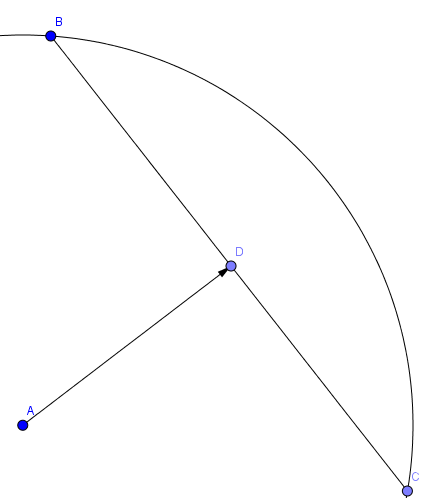
\includegraphics[width=0.3\linewidth]{images/quatrot1} 
	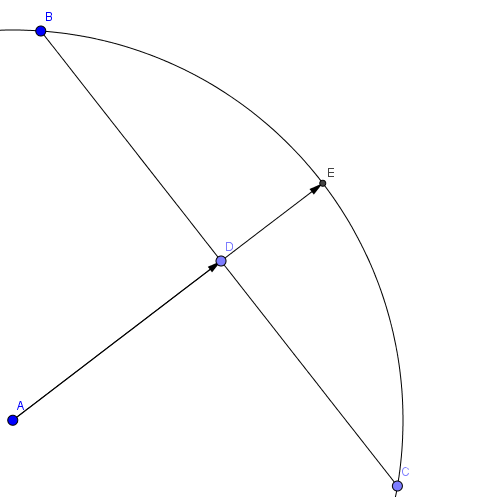
\includegraphics[width=0.33\linewidth]{images/quatrot2} 
	\caption{\label{fig:image} On the left: Idea, how linear interpolation between rotation matrices looks. If linear interpolation between the two points $B$ and $C$ on a circle is used, the resulting point does not lie on the circle. On the right: Interpolating with quaternions. The result can be easily mapped onto the sphere by normalizing the quaternion.
	}
\end{figure}


\subsection{Recap Skinning}
Now we have a method to deform meshes with the help of bones and to blend in given example poses.
The input consists of the constant data:
\begin{itemize}
	\item The Vertex positions in undeformed state: $\bm u\in\mathbb{R}^{N\times 3}$
	\item The weighting of each bone for the vertcies: $\bm W\in\mathbb{R} ^{N \times B}$
	\item The transformation for each example pose and bone, consisting of
	\subitem The rotational part $\bm R\in\mathbb{R}^{B\times 4\times  E}$
	\subitem The translational part $\bm T\in\mathbb{R}^{B \times 3\times E}$
\end{itemize}
and the changing data:
\begin{itemize}
	\item example Weights $\bm{E}\in\mathbb{R}^{N\times E}$
\end{itemize}
Let $\text{rotate} (\bm{q},\bm{x})$ be the function that rotates the position $\bm{x}$ by the quaternion $\bm{q}$.
The translational part is interpolated linearly, the rotational by the $QLERP$-algorithm.
The skinned mesh vertex positions $\bm{x} \in \mathbb{R}^{N\times 3}$ can now be calculated by:
\begin{align}
\label{form:blend}
\bm{x}_i = \sum_{b\in B} \bm{W}_{ib}\left(\sum_{e=1}^{E}\bm{E}_{ie}\bm{T}_{be} + \text{rotate}(\text{QLERP}(\bm{E}_i,\bm{R}_b),\bm{u}_i)\right)
\end{align}

\subsection{Calculate example weighting}
When two objects collide, the rigid body simulator passes the vertex $\bm{x}_i$, where the collision occurred and the impulse $\bm{j}_i$.
The goal is now to calculate a 	useful change $\bm{\Delta E}$ of the example weights, that matches the impact. They are later applied to the example weight matrix $\bm E$. Initially every entry of the first column of $\bm E$ contains 1 and the rest is 0. The first column represents the weighting of the undeformed mesh. That means the mesh is undeformed at the beginning. As example poses are used, not every deformation is possible. So we first calculate an ideal deformation for the vertex being hit. Then we solve a minimization problem, trying to get good example weightings, so that the distance between the ideal deformation and the skinned position of the vertex is minimal. Afterwards we propagate this change to the vertices around.
\subsubsection{Projection}
We want to compute the desired position based on the impulse, given to us by the rigid body simulator. Impulse is a change in momentum. So we can write:
\begin{align}
\bm j = m \bm v
\end{align}
To get the change in position of the object in the next timestep, we divide by the mass and multiply by the duration of the timeslice:
\begin{align}
\bm{\Delta x}= \frac{\Delta t}{m} \bm j
\end{align}
To prevent deformation on contact and on soft impacts we add a threshold $\beta$, which prevents the object from deforming to easily and takes out some of the energy. We end up with the following formula for the impacted vertex:
\begin{align}
\bm{\Delta x}_i = \frac{\Delta t}{m} \max(||\bm{j}_i|| - \beta, 0) \frac{\bm j_i}{||\bm j_i||}
\end{align}

We now construct the Jacobian matrix $\bm J$ by differentiating formula \ref{form:blend}. This is done with help of automatic differentiation \cite{autoDiff}. The matrix contains all partial derivatives of 
\begin{align}
\bm J_i &= \frac{\partial\bm x_i}{\partial \bm E_{ie}} \in \mathbb{R}^{3\times E}
\end{align}
\begin{align}
&=
\begin{pmatrix}
\frac{\partial\bm x_{i1}}{\partial \bm E_{i1}} &...&\frac{\partial\bm x_{i1}}{\partial \bm E_{in}} &...&\frac{\partial\bm x_{i1}}{\partial \bm E_{iE}} \\
\frac{\partial\bm x_{i2}}{\partial \bm E_{i1}}&&\frac{\partial\bm x_{i2}}{\partial \bm E_{in}}&&\frac{\partial\bm x_{i2}}{\partial \bm E_{iE}}\\
\frac{\partial\bm x_{i3}}{\partial \bm E_{i1}} &...&\frac{\partial\bm x_{i3}}{\partial \bm E_{in}} &...&\frac{\partial\bm x_{i3}}{\partial \bm E_{iE}} \\
\end{pmatrix}
.
\end{align}
It contains the change in vertex position depending on a change in the example weighting. So given a change of position $\bm{\Delta x}$, in the example space we can compute the change of example weightings by:
\begin{align}
\bm{\Delta e}_i &= \bm J_i^T \bm{\Delta x}_i\\
\begin{pmatrix}
\Delta e_{i1} \\
...\\
\Delta e_{in} \\
...\\
\Delta e_{iE} \\
\end{pmatrix}
&=
\begin{pmatrix}
\frac{\partial\bm x_{i1}}{\partial \bm E_{i1}} &\frac{\partial\bm x_{i2}}{\partial \bm E_{i1}}&\frac{\partial\bm x_{i3}}{\partial \bm E_{i1}}\\
...&&...\\
\frac{\partial\bm x_{i1}}{\partial \bm E_{in}}&\frac{\partial\bm x_{i2}}{\partial \bm E_{in}}&\frac{\partial\bm x_{i3}}{\partial \bm E_{in}}\\
...&&...\\
\frac{\partial\bm x_{i1}}{\partial \bm E_{iE}}&\frac{\partial\bm x_{i2}}{\partial \bm E_{iE}}&\frac{\partial\bm x_{i3}}{\partial \bm E_{iE}}\\
\end{pmatrix}
\begin{pmatrix}
\Delta x_{i1}\\
\Delta x_{i2}\\
\Delta x_{i3}\\
\end{pmatrix}
\end{align}
This formula however requires the change to be in the space of possible changes, that can be achieved by the examples. Our goal is now to get a good value for the change in example weights $\bm{\Delta e}$. To achieve that we have to get the change, that happens, if we apply $\bm{\Delta e}$ as close as possible to the desired change $\bm{\Delta x_i}$. Let $\bm x_i(e)$ be the function that moves the vertex according to the example weighting $e$. Then we have to solve:
\begin{align}
\bm{\Delta e} = \min_{\bm{\Delta \hat e}}||(\bm x_i (\bm e + \bm{\Delta \hat e}) -\bm x_i (\bm e )) - \bm{\Delta x}_i ||^2
\end{align}

A method to solve minimization problems is the method of steepest descent. It uses the fact that a gradient always points in the opposite direction of the steepest descent. So if we start at some point and follow the direction of the gradient in infinite many, infinitesimal small steps we reach a local minimum, as far as it exists. Similar to a marble rolling around on a surface. It will sometime reach a lokal minimum, as it always follows the direction of steepest descent. Of course the marble has to be somewhat sticky, otherwise its momentum would prevent it from following the gradient directions.\\
Instead of going infinite small steps we take finite many not so small steps.
As we do not opt for physical accuracy it is sufficient to go one step. As initial value $\bm{\Delta e} = 0$ is used. This makes the first term of the minimization cancel out. The gradients can by definition be calculated by transposing the Jacobi matrix:
\begin{align}
\bm J_i^T \bm{\Delta x}_i
\end{align}
is the gradient on $\Delta x$.

The stepwidth of the step is chosen, so that it is dependent on the impact and user controllable: $\alpha ||\bm{\Delta x}||$
The approximated change in Example weightings is calculated by:
\begin{align}
\bm{\Delta e}_i = \alpha ||\bm{\Delta x}|| \frac{\bm J_i^T \bm{\Delta x}_i}{||\bm J_i^T \bm{\Delta x}_i||}
\end{align}

\subsection{Propagation}
By now we only calculate a change of example weights for one vertex. In order for the result to look acceptable, the change has to be propagated nearby vertices. To calculate the distance between two vertices, Dijksta's algorithm is used. The change of Example weights for every vertex is saved in the Matrix $\bm{\Delta E}$. To propagate the change we modify each column by:
\begin{align}
\bm{\Delta E}_j \;+\!\!= \phi\left(\frac{\text{dist}(\bm x_j , \bm x_i)}{\gamma}\right) \bm{\Delta e}_i\\
\phi(x) =
\begin{cases}
2x^3 - 3x^2 + 1 & : x< 1\\
0               & : otherwise	
\end{cases}
\end{align}
The function $\phi$ is called kernel smoother. It assures that the change is applied fully on the impacted vertex. With increasing distance the extend of application decreases. How far the changes should be propagated is determined by the value $\gamma$.
\subsection{Application of the Deformation}
To let the impact look more natural, the deforming does not happen instantaneously, but over time. The Matrix $\bm{\Delta E}$ contains the change in example weighting that still has to be applied. Every timestep a bit of the deformation accumulator  $\bm{\Delta E}$ is applied and decreased by the same amount. This is achieved through the user given parameter $\lambda$.
\begin{align}
\bm E \;+\!\!= (1-\lambda)\bm{\Delta E} \\
\bm {\Delta E} \;*\!\!= \lambda
\end{align}
Note that the amount of application is high directly after the impact and decreases over time. For $t\rightarrow\infty$ the whole change is applied.
\subsection{Restitution Modifiaction}
As a deformation consumes energy it is necessary to show this in the movement of the object. With the deformation the nonelastic part of the collision increases. The ratio between the elastic and non-elastic part, the coefficient of restitution is modified by:
\begin{align}
C_r := \min(C_r^*, C_r + \mu \Delta t, \exp(-\nu||\bm{\Delta E}||_f)C_r^*)
\end{align}
The first term $C_r^*$ is the coefficient that is initially used by the rigid body simulator. The second term increases over time to avoid jittering and the third parameter decreases over time. $\mu$ and $\mu$ are user given parameters.



\subsection{Userparameters}
The following parameters are adjustable by the user and determine:
\begin{itemize}
	\item $\alpha$: how much the impact deforms the bodies
	\item $\beta$: how strong the impact has to be to be noticed
	\item $\gamma$: how far the deformation is propagated
	\item $\lambda$: how long the deformation should take
	\item $\mu$ and $\nu$: how elastic the collision is modified
\end{itemize}
\subsection{Fracture}
Fracturing of the mesh is supported. During design time the artist splits up the mesh into individual parts. 
The parts are hold together by constraints. If a force exceeds a threshold the contraints are removed and the model is fractured.
\section{Discussion and Conclusion}
\subsection{Conclusion}
The method described provides an efficient solution to plastic deformations. It is based on example deformations. So the user has intuitive control over how the deformed meshes look. It uses a rigid body simulator and only deformes the objects on impact. So the speed of rigid body simulators is combined with the ability to simulate plastic deformation. Experiments have shown that very few example poses are sufficient to get fairly realistic looking results. It is not necessary to provide hundreds of examples for each mesh.
\subsection{Performance}
Using the method to simulate deformation adds a avarage of 42\% to 59\% of the initial computing time to every timestep in the tests. It is significantly slower than regular rigid body simulation. One reason for this is the collision detection. There are very efficient alogrithms to calculate collisons on convex bodies. To use them on arbitrary meshes, the meshes are split up to convex parts. As the shape of the objects changes during the method the splitting cannot be precomputed. So the collision has to be detected for non convex bodies, which is less efficient.\\
Although the method is slower than usual rigid body simulation it still is extremely efficient, compared to other methods for computing plastic deformations as the finite element method or spring mass systems.
\subsection{Future Work}
A possible improvement would be automated rigging. Then example poses can be provided by soft body simulators and integrated into the system.\\
Implementing an application for modeling the objects or integrating a plugin for a given application would give the possitility to modify parameters with brushes individually for the vertices.



\bibliographystyle{alpha}
\bibliography{references}

\end{document}          
